\documentclass{beamer}
\mode<presentation> {


\usetheme{Madrid}

}
\usepackage{booktabs}
\usepackage[utf8]{inputenc}
%\usepackage[spanish, mexico]{babel}
\usepackage{listings}
\usepackage{breakcites}
\usepackage{dsfont}
\usepackage{hyperref}
\usepackage{amssymb,amsthm,amsmath,latexsym}
\usepackage{natbib}
\theoremstyle{plain}
\newtheorem{teo}{Theorem}
\newtheorem{prop}[teo]{Proposition}
\newtheorem{defi}[teo]{Definition}
\newtheorem{obs}[teo]{Observation}
\newtheorem{lem}[teo]{Lemma}
\newtheorem{cor}[teo]{Corolary}
\usepackage{tikz}
\usetikzlibrary{trees}
\usetikzlibrary{calc}


%----------------------------------------------------------------------------------------
%	TITLE PAGE
%----------------------------------------------------------------------------------------

\title[Causally Choosing]{Use and acquisition of causal knowledge in a decision making process} % The short title appears at the bottom of every slide, the full title is only on the title page

\author{Mauricio Gonzalez Soto} % Your name
\institute[INAOE] % Your institution as it will appear on the bottom of every slide, may be shorthand to save space
{
Instituto Nacional de Astrofísica Óptica y Electrónica \\ % Your institution for the title page
\medskip
\textit{mauricio@inaoep.mx} % Your email address
}
\date{\today} % Date, can be changed to a custom date

\begin{document}

\begin{frame}
\titlepage % Print the title page as the first slide
\end{frame}

\begin{frame}[allowframebreaks]
\frametitle{Contents} % Table of contents slide, comment this block out to remove it
\tableofcontents[hideallsubsections] % Throughout your presentation, if you choose to use \section{} and \subsection{} commands, these will automatically be printed on this slide as an overview of your presentation
\end{frame}

%
%\begin{frame}
%    \frametitle{Outline}
%    \begin{columns}[t]
%        \begin{column}{.3\textwidth}
%            \tableofcontents[sections={1-3}]
%        \end{column}
%        \begin{column}{.3\textwidth}
%            \tableofcontents[sections={4-5}]
%        \end{column}
%         \begin{column}{.3\textwidth}
%            \tableofcontents[sections={6-9}]
%        \end{column}
%    \end{columns}
%\end{frame}

%--------SLIDES------------------------------

\section{Introduction}
\subsection{General Overview}
\begin{frame}
\frametitle{General Idea}
\begin{itemize}
\item We live in a causally structured world. 
\item Our actions \textit{cause} changes in the environment.
\item We consider this changes in order to plan our actions when facing similar situations.
\end{itemize}
\end{frame}

\begin{frame}
\frametitle{Human use of Causal Relations}
\begin{itemize}
\item \cite{hagmayer2013repeated} show how human beings use and modify causal information.
\item Both \cite{hohwy2013predictive}, \cite{clark2015surfing}, assert that the brain itself is a causal hypothesis tester. 
\item While Danks \cite{danks2014unifying} argues that cognitive processes (including causal reasoning) take place in the mind as graphical models, Tenenbaum's school argues that the mind uses hierarchical bayesian inference (\cite{kemp2010learning}).
\end{itemize}
\end{frame}

\begin{frame}
\frametitle{Our setting}
\begin{itemize}
\item Consider a \textit{rational} decision maker in an uncertain environment.
\item Consequences of actions can not be predicted.
\item We add an extra to the environment: causal structure.
\item This means that there exists a fix but unknown causal model that governs the environment where the agent lives.
\end{itemize}
\end{frame}

\begin{frame}
\frametitle{A brief on causal models}
\begin{itemize}
\item Causal models encode cause-effect relations. 
\item Relations are encoded in a graph.
\item Can be used to predict \textit{effects} of certain causes without necessarily performing the action.
\item They allow to \textit{imagine} what would happen if...
\end{itemize}
\end{frame}

\begin{frame}
\frametitle{Causal Model: Example}
\begin{figure}[ht]
\vskip 0.2in
\begin{center}
\includegraphics[width=\linewidth]{/Users/MauricioGS1/INAOE/Propuesta/presentacion/example.png}
\end{center}
\vskip -0.2in
\end{figure}
\end{frame}

\begin{frame}
\frametitle{Our Proposal}
\begin{itemize}
\item Current decision-making theories do not consider causal structure in decision making processes
\item We \textbf{propose} an autonomous rational agent who can use and learn causal information while interacting with its environment.
\end{itemize}
\end{frame}

\section{Concepts}
\begin{frame}
\frametitle{Concepts}
Concepts and Framework:
\begin{enumerate}
\item Causal Models.
\item Decision Problems.
\end{enumerate}
\end{frame}

\subsection{Causal Models}
		\begin{frame}
		\frametitle{Causal Models}
		Causality and Causal Models:
		\end{frame}
		\begin{frame}
		\frametitle{Difference between causal and associative relations}
		\begin{itemize}
		\item With associative relations we can't figure out what influenced (or caused) what.
		\item Consider this: A distribution $p(a,t)$ can be factored both as $p(a|t)p(t)$ and $p(t|a)p(a)$. 
		\item In terms of a Bayesian Network, $T \to A$, and $A \to T$, but both can't be causal.
		\item Causal relations need not be in temporal order: consider a barometer and a storm.
		\end{itemize}
		\end{frame}
		
		\begin{frame}
		\frametitle{Formal Definition of Causality according to \cite{spirtes2000causation}}
		\begin{defi}
		Let $(\Omega, \mathcal{F}, \mathbb{P})$ a finite, probability space and consider a binary relation  $\to  \subseteq \mathcal{F} \times \mathcal{F}$ such that
		\begin{itemize}
		\item Transitive: if $A \to B$ and $B \to C$ for $A,B,C \in \mathcal{F}$ then $A \to C$.
		\item  Irefflexive: for each $A \in \mathcal{F}$ it is not true that $A \to A$.
		\item Antisymetric: for $A, B \in \mathcal{F}$, if $A \to B$, then it is not true that $B \to A$.
		\end{itemize}
		If $A \to B$ we will say that $A$ is \textbf{a cause} of $B$.
		\end{defi}
		\end{frame}
		
		\begin{frame}
		\frametitle{From Graphs to Probability Measures}
		Given a Directed Acyclic Graph, one can build the probability distribution $P_\mathcal{G}$ that expresses the relations of the graph (\cite{koller2009probabilistic}). \\
		We require, as axioms, that this measure satisfies:
        \begin{itemize}
        \item Causal Markov Condition.
        \item Causal Minimality.
         \item Causal Faithfulness.
         \item Causal Sufficiency
        \end{itemize}
		\end{frame}
		
	\begin{frame}
	\frametitle{Causal Graphical Models}
	\begin{defi}
	A causal graphical model (\cite{spirtes2000causation}, \cite{pearl2009causality}, \cite{koller2003multi}, \cite{sucar2015probabilistic}) consists of:
	\begin{itemize}
	 \item A set of random variables $\mathcal{X}=\{ X_1,...,X_n \}$.
	 \item A directed acyclic graph (DAG) $\mathcal{G}$.
	 \item An operator $do()$ defined over the space of DAG's whose action consists of: given $\mathbf{X} \subseteq \mathcal{X}$ and $\mathbf{x} = \{ x_{i_1}, x_{i_2}, ... , x_{i_j} \} \in Val(\mathcal{X})$, then $do(\mathbf{X} = \mathbf{x} )$ assigns to each $X_j \in \mathbf{X}$ the value $x_{i_j}$ and deletes any incoming edge on it.
	 \end{itemize}
	 \end{defi}
	 \end{frame}

\subsection{Decision Problems}
	\begin{frame}
	Decision Problems and Rational Thinking.
	\end{frame}
	\begin{frame}
	\frametitle{Decision Problems}
	A decision problem is composed by (\cite{bernardo2000bayesian}, \cite{gilboa2009decision}):
	\begin{itemize}
	\item A set of available options $\mathcal{A}$.
	\item A (rational) decision maker with preference relation $\succeq$ defined over $\mathcal{A} \times \mathcal{A}$.
	\item A family of uncertain events $\mathcal{E}$.
    \item A family of possible outcomes $\mathcal{C}$
	\end{itemize}
	\end{frame}
	
	\begin{frame}
	\frametitle{Choosing rationally}
	Savage's Theorem (\cite{savage1954the}) says that:
\begin{teo}	
	If a rational decision maker does not know the probabilities of uncertain events ocurring, then he must choose according to the expected utility with respect to a \textit{subjective} probability measure and a \textit{subjective} utility function.
\end{teo}
Details can be found at \cite{bernardo2000bayesian}, \cite{gilboa2009decision}.
	\end{frame}

\section{Research Problem}
\begin{frame}
About my Proposed Research:
\begin{enumerate}
\item Motivation.
\item Justification.
\item Research Questions.
\item Problem Statement.
\item Hypothesis.
\end{enumerate}
\end{frame}
	\subsection{Motivation}
	\begin{frame}
	\frametitle{Motivation: 1}
	\begin{itemize}
	\item Decision making under uncertain conditions is a fundamental part of intelligent reasoning (\cite{lake2017building}).
	\item Intelligent agents often face situations where an action must be chosen in the presence of uncertain conditions.
	\end{itemize}
	\end{frame}
	\begin{frame}
	\frametitle{Motivation: 2}
	\begin{itemize}
	\item It is known that human beings conceive their actions on the world as \textit{intervening} in the world (\cite{hagmayer2009decision}).
	\item Following this idea, \cite{lattimoreNIPS2016} consider decision problems where the action to be chosen is an intervention over a known causal graphical model.
	\item What about \textbf{not knowing} the causal model? 
	\end{itemize}
	\end{frame}
	
	\subsection{Justification}
	\begin{frame}
	\frametitle{Justification: Un-interpretable models}
	\begin{itemize}
	\item Many real-world applications of decision making are solved by \textit{associative} methods.
	\item Associative methods capture only statistical patterns that are found in data.
	\item As an example, methods based in Deep Neural Networks aren't even supposed to explain why a certain output was produced since those methods are based in \textit{parallel distributed representations}.
	\end{itemize}
	\end{frame}
	
	\begin{frame}
	\frametitle{Justification: Need for interpretable decision-making models}
	\begin{itemize}
	\item Current methods for Decision Making are based in Reinforcement Learning, and specifically in Deep Reinforcement Learning. 
	\item Although good performance in the task, they can not explain \textit{why} a specific trajectory was chosen by the algorithm.
	\item This is highly relevant in real-world applications such as self-driving cars.
	\end{itemize}
	\end{frame}
	
	\begin{frame}
	\frametitle{Justification: Explaining why}
	\begin{itemize}
	\item On the other hand, learning a causal model of an environment and using it to act upon the environment allows to \textit{explain} aspects of the model that a purely associative model would not be able to explain. 
	\item It allows to ask \textit{why}.
	\item Transferability
	\end{itemize}
	\end{frame}

	\subsection{Research Questions}
	\begin{frame}
	\frametitle{Research Questions}
	The proposed research is ultimately trying to answer a series of questions about the nature of causal relations and about their possible use.
	\begin{enumerate}
	\item How a rational decision maker who faces an uncertain environment which is governed by a causal mechanism can learn and make use of this causal structure in order to make good    	choices? 
	\item How can a causal structure help a decision maker in order to guide his learning process? 
	\item What does the rationality assumption implies about how to choose when considering causal information? 
\item How to trade off exploration and exploitation when trying to learn about the causal structure of an environment while also trying to make good choices?
\end{enumerate}
\end{frame}

\subsection{Statement}
	\begin{frame}
	\frametitle{Problem Statement}
	\begin{itemize}
	\item Let  $\mathcal{G}$ a causal graphical model.
	\item Let $(\mathcal{A},\mathcal{E},\mathcal{C})$ a decision problem under uncertainty whose actions $a_i = \{ c_j | E_j : j \in J \}$  are causally related to consequences $c \in \mathcal{C}$ through the uncertain events $E \in \mathcal{E}$ which correspond to variables in $\mathcal{G}$. 
	\item Consider a rational decision maker who doesn't know the causal model which control the probabilities of observing a consequence given an action $a \in \mathcal{A}$.
	\item We ask how the decision maker could learn about the causal structure that controls his environment in order to make good choices with respect to the decision makers' preferences.
	\end{itemize}
	\end{frame}

	\subsection{Hypothesis}
	\begin{frame}
	\frametitle{Hypothesis}
	\begin{itemize}
	\item Let $\mathcal{G}$ a causal graphical model and let $(\mathcal{A},\mathcal{E},\mathcal{C})$ a decision problem whose actions $a_i = \{ c_j | E_j : j \in J \}$  are causally related to consequences $c \in \mathcal{C}$ through the uncertain events $E \in \mathcal{E}$ which correspond to variables in $\mathcal{G}$.
	\item Then, if a decision maker doesn't know the probabilities of the uncertain events in $E$, by repeatedly making decisions he can learn a causal model of the environment and use it to find the optimal action (in the sense of expected utility theory) in less, or equal, rounds than if he doesn't consider causal information.
	\end{itemize}
	\end{frame}

\section{Approaches and Related Work}
\begin{frame}
\frametitle{Approaches and Related Work}
Approaches and Related Work:
\end{frame}
\begin{frame}
\frametitle{Approaches and Related Work}
\begin{figure}[ht]
\vskip 0.2in
\begin{center}
\includegraphics[width=\linewidth]{/Users/MauricioGS1/INAOE/Propuesta/presentacion/Related_Work.png}
\caption{Related Work}
\end{center}
\vskip -0.2in
\end{figure}
\end{frame} 

\subsection{Approaches and Related Work: Reinforcement Learning}
\begin{frame}
\frametitle{Reinforcement Learning (RL)}
\begin{itemize}
\item Reinforcement Learning uses only associative patterns for finding an optimal policies.
\item Optimal policies actually achieve the maximum expected utility as required by the rationality condition (\cite{webb2007game}).
\item In this way, when only associative information is available, RL is a coherent learning framework. 
\end{itemize}
\end{frame}

\subsection{Approaches and Related Work: Causal learning in humans}
\begin{frame}
\frametitle{Causal Learning in Human beings}
\begin{itemize}
\item Human beings, while facing a sequential decision problem, use and modify causal information.
\item \cite{hagmayer2009decision}, \cite{hagmayer2013repeated} show that human beings can learn causal information in simple decision-making tasks, but remains open to study causal learning while seeking for a specific objective. 
\end{itemize}
\end{frame}
\subsection{Approaches and Related Work: Joyce's Causal Decision Theory}
\begin{frame}
\frametitle{Joyce's Causal Decision Theory}
\begin{itemize}
\item An attempt to formalize Decision Theory in the presence of Causal Information was attempted by Joyce (\cite{joyce1999foundations}), who stated that a decision maker must choose whatever action is more likely to (causally) produce desired outcomes.
\item  His formulation falls short since he does not consider any kind of formal causal model beyond what is commonly understood by causality
\end{itemize}
\end{frame}
\subsection{Approaches and Related Work: Bandits}
\begin{frame}
\frametitle{Bandits: Non-causal}
\begin{itemize}
\item In the class of decision problems considered for this proposal it is assumed that the a rational agent must choose some available action and then receive a reward from it.
\item Problems of this nature have been modelled as \textit{bandit} problems.
\item Best-arm algorithms exist: none consider causal information.
\end{itemize}
\end{frame}
\begin{frame}
\frametitle{Bandits: Causal bandits}
\begin{itemize}
\item An action can be conceived as an \textit{intervention} over an environment, which is in fact how humans consider their actions in the world.
\item They use and modify causal knowledge during a sequential decision making process.
\item It is shown by \cite{lattimoreNIPS2016} that adding causal information in a fixed budget decision problem allows the decision maker to learn \textit{faster} had he not considered causal information.
\item Their work requires that the causal model is fully known to the decision maker.
\item Relaxed later by \cite{sen2017identifying} who requires only that some part of the causal model is known and allow interventions over the unknown part. 
\end{itemize}
\end{frame}
\section{Proposed Solution and Methodology}
\begin{frame}
\frametitle{Proposed Solution and Methodology}
Proposed Solution and Methodology:
\begin{enumerate}
\item General and Specific Objectives.
\item Methodology.
\item Validation.
\item Detailed Methodology.
\end{enumerate}
\end{frame}

	\subsection{Objectives}
	\begin{frame}
	\frametitle{General Objectives}
	The proposed research has as a general objective:
	\begin{itemize}
 \item Understand the implications of causality for rational decision maker who faces an uncertain environment and how causal relations can be discovered and used in order to make good choices that maximize the expected utility for the decision maker.
	\end{itemize}
	\end{frame}
	
	\subsection{Specific Objectives}
	\begin{frame}
	\frametitle{Specific Objectives}
	In order to reach the General Objective we must:
	\begin{enumerate}
	\item Define a Game between agent and Nature in order to model agent-environment interaction.
	\item Find an adequate family of probability distributions that encode causal knowledge.
	\item Develop a general belief-updating criteria in terms of causal information.
	\end{enumerate}
	\end{frame}

\subsection{Methodology}
\begin{frame}
\frametitle{Proposed Solution: Conceptual step-by-step methodology}
\begin{itemize}
\item Rational agent in a causal environment.
\item Modelling agent-environment interaction as a \textit{game}.
\item Encoding current causal knowledge as probabilsitic \textit{beliefs}
\item Using current knowledge to make a choice.
\item Updating causal information.
\end{itemize}
\end{frame}

\subsection{Validation}
\begin{frame}
\frametitle{Validation}
How to know if objective has been achieved?
\end{frame}

\begin{frame}
\frametitle{Concurrent Validation}
We will be comparing against standard Reinforcement Learning methods such as Q-Learning (\cite{watkins1992q}) since it has been shown that optimal policies achieve the objective of Max Expected Utility.
\end{frame}

\begin{frame}
\frametitle{A conjecture}
It needs to be shown that given the rewards obtained by a decision-making procedure that achieves the MEU, then my proposed algorithm must stay close to it.
\begin{teo}
Let $(X_1,X_2,...)$ the rewards obtained by a decision-making procedure which is known to converge to the max expected utility (or an optimal policy), then, if $(Y_1, Y_2,...)$ are the rewards obtained by a decision-making procedure that uses causal information in the way we propose, then for all $\varepsilon > 0$ there exists an $N_\varepsilon \in \mathbb{N}$ such that $ | X_t - Y_t | < \varepsilon$ for any $t > N_\varepsilon$. 
\end{teo}
\begin{proof}
To be proved.
\end{proof}
\end{frame}

\begin{frame}
In this case, if we succeed in finding an action whose reward equals that of RL algorithms, then we will have chosen the optimal action using Causal Information as proposed in the Hypothesis.
\end{frame}

\begin{frame}
\frametitle{How to}
How to
\end{frame}

\subsection{Proposed Solutuion: A guiding principle}
\begin{frame}
\frametitle{A guiding principle for Causal Decision Problems}
We propose the following principle as a normative guide for how causal information must be used in order to find a solution to a decision problem where the preferences of the decision maker are assumed to be rational.\\
We consider only the case where the decision maker's utility is given by the outcome of a $\{0,1 \}$-binary variable.\\
It remains to be refined and extended for a general case. 
\end{frame}

\begin{frame}
\begin{prop}
Let  $\mathcal{G}$ a causal graphical model and let $(\mathcal{A},\mathcal{E},\mathcal{C})$ a decision problem under uncertainty whose actions $a_i = \{ c_j | E_j : j \in J \}$  are causally related to consequences $c \in \mathcal{C}$ through the uncertain events $E \in \mathcal{E}$ which correspond to variables in $\mathcal{G}$. Let $Y$ a variable in $\mathcal{G}$ the variable whose realizations correspond to the consequences of the decision problem once the agent has chosen an action $a \in \mathcal{A}$ and assume that $Y$ only takes values in the set $\{ 0,1\}$ where $1$ is a more desired outcome for the agent. Then, the $\textit{solution}$ for this decision problem is given by the action $a^\ast \in \mathcal{A}$ that satisfies:
\[ P(Y=1 | do(a^\ast)) \geq P(Y=1 | do(a)) \textrm{ for all } a \in \mathcal{A}. \]
\end{prop}
\end{frame}

\subsection{First Step: Modelling a Causal Decision Problem as a Game}
\begin{frame}
\frametitle{First Step: Modelling a Causal Decision Problem as a Game}
\begin{itemize}
\item The next step is to model the interaction of the (original) decision maker and his environment as a \textbf{game} between two players: 
\begin{enumerate}
\item The (original) decision maker.
\item A player which will be called \textbf{Nature}, whose actions are to be guided by the causal model.
\item The game is over when the \textit{outcome} of the original decision problem is realized. This we will call a \textit{round}.
\end{enumerate}
\end{itemize}
\end{frame}

\begin{frame}
\begin{itemize}
\item  We assume that player Nature has the first move and she assigns some state to any, or all, of the variable(s) in the causal model $\mathcal{G}$.
\item After the decision maker makes his \textit{play}, Nature will \textit{respond} to the action selected according to the causal relations expressed by $\mathcal{G}$.
\item This action-response dynamic forces to consider some notion of order between the players' moves, and because of this reason we must use the \textit{extensive-form} games. Details in \cite{osborne1994course}.
\end{itemize}
\end{frame}

\subsection{Second Step: Belief formation}
\begin{frame}
\frametitle{Second Step: Belief Formation}
\begin{itemize}
\item The whole idea is that a decision maker is able to \textbf{learn} and \textbf{reason} about his environment by observing the effects of his actions.
\item The agent encodes any previous knowledge or uncertainties in a probability distribution.
\item The observed information will be used to modify his current knowledge in a way that is similar to how human beings modify causal knowledge while intervening in the world
\end{itemize}
\end{frame}

\subsection{Third Step: Making choices}
\begin{frame}
\frametitle{Third Step: Making Good Choices}
\begin{itemize}
\item The decision maker uses his current knowledge \textit{as if} it were the truth about the causal relations of his environment.
\item With this information he will choose the action that maximize the Expected Utility, according with our guiding principle.
\end{itemize}
\end{frame}

\subsection{Fourth Step: Belief updating}
\begin{frame}
\frametitle{Belief Updating}
\begin{itemize}
\item It is known that belief updating using Bayes' Theorem is the only way rational way of updating uncertainty.
\item It remains to be answered how to concretely use causal information in order to update the parameters that control the distributions used to express beliefs in a tractable way.
\end{itemize}
\end{frame}

\section{Methodology divided into simpler cases}
\begin{frame}
We will show how the methodology applies in simpler and easier cases where the decision maker has some extra info about his environment.
\end{frame}
\subsection{Fully knowing the causal graphical model}
\begin{frame}
\frametitle{Fully knowing the causal graphical model}
\begin{itemize}
\item Following the guiding principle, he could easily calculate the effect on the target variable that any of his actions has.
\item Choose the action that has the highest probability of causing a \textit{desired} value of the target variable.
\end{itemize}
\end{frame}

\subsection{Knowing only the graph structure}
\begin{frame}
\frametitle{Knowing only the causal graph structure}
\begin{itemize}
\item The agent encodes uncertainty over the parameters of the model as a probability distribution over a suitable space.
\item Done in such way that a \textit{local} (i.e. in each round) causal model can be obtained from current beliefs in order to make a decision using current causal knowledge.
\item The agent forms a causal model which is used as, according to the guiding principle, as if it were the true causal model.
\item Belief updating.
\end{itemize}
\end{frame}

\subsection{General case: Model unknown}
\begin{frame}
\frametitle{Model unknown}
If the model is completely unknown, two ideas appear:
\begin{enumerate}
\item If the maximum number of variables is known.
\item If it is not.
\end{enumerate}
\end{frame}
\begin{frame}
\frametitle{Idea 1 for the General Case}
\begin{itemize}
\item If the maximum number of variables is assumed to be known by the decision maker, then the situation simplifies since a decision maker could generate distributions that represent causal relations among variables.
\item For example, a Dirichlet Process (\cite{ferguson1973bayesian}, \cite{ghosal2017fundamentals}) could be used to generate Dirichlet distributions that are used generate Conditional Probability Tables in order to specify a causal model as in the previous case.
\end{itemize}
\end{frame}

\begin{frame}
\frametitle{Idea 2 for the General Case}
\begin{itemize}
\item If the number of variables is unknown, then the beliefs that the decision maker holds must allow unbounded cardinality on the number of variables. 
\item In that case, a distribution over a \textit{graph space} could be used in such a way that when sampled a graph structure is obtained and used as in the previous case.  
\item The graph generating process must converge to the true model.
\end{itemize}
\end{frame}

\section{Working and Publications Plan}
\begin{frame}
Working and Publications Plan
\end{frame}
\subsection{Working Plan}
\begin{frame}
\frametitle{Working Plan}
\begin{enumerate}
\item Literature Review.
\item Studying implications of the rationality assumption for decision making under uncertainty in causal environments.
\item Formalization of a Causal Decision Problem.
\item Propose a representation of beliefs that allow causal structure to be considered.
\item Propose and evaluate an updating criteria for causal beliefs that can be updated according to new information when involved variables are known.
\item Study the problem of on-line causal discovery (fully unknown model). Convergence of proposed solution.
\end{enumerate}
\end{frame}

\subsection{Publications Plan}
\begin{frame}[allowframebreaks]
\frametitle{Publications Plan}
\begin{itemize}
\item \textbf{Year 1:} Gonzalez-Soto, M., Sucar, L.E., Escalante, H.J., \textbf{Playing against Nature: causal discovery for decision making under uncertainty}. Presented at \textbf{CausalML 2018 Workshop at ICML 2018}. July 15 2018, Stockholm, Sweden. The paper can be found at \url{https://arxiv.org/abs/1807.01268}.
\item \textbf{Year 2:} Conference Paper 2 
		\begin{itemize}
		\item The implications of Causal Relations for Decision Making: a general principle for Decision under Uncertainty.
		\item Possible Forum: \textbf{Beyond Curve Fitting: Causation, Counterfactuals, and Imagination-based AI. AAAI Spring Symposium}, March 25-27, 2019, Stanford, CA
		\end{itemize}
\item \textbf{Year 2:} Conference Paper 3 
	\begin{itemize}
	\item When a causal model is unknown but the involved variables are known, how to encode uncertainties about causal structure in a probabilistic distribution? Bayesian Nonparametric prior that explicitly represents causal structure.
	\item When variables of the environment are unknown how to encode prior beliefs and how to update them when data is not fully observed.
	\item Possible Forum: International Conference on Bayesian Nonparametrics, International Conference on Probabilistic Graphical Models.
	\end{itemize}
\item \textbf{Year 3:} Journal Paper
		\begin{itemize}
			\item Aim: Theoretical paper of results for on-line causal learning.
		\end{itemize}
\end{itemize}
\end{frame}

\begin{frame}
\frametitle{Gantt Diagram}
\begin{figure}[ht]
\vskip 0.2in
\begin{center}
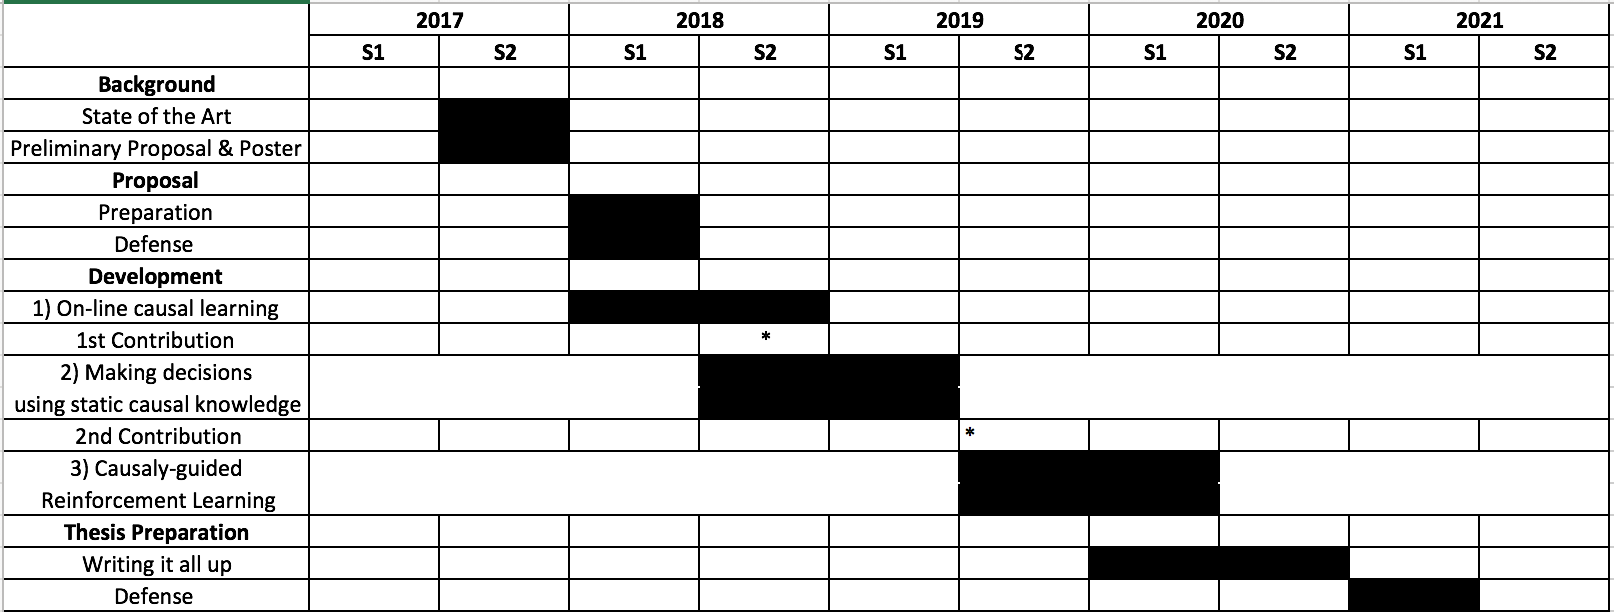
\includegraphics[width=\linewidth]{/Users/MauricioGS1/INAOE/Propuesta/presentacion/Gantt.png}
\end{center}
\vskip -0.2in
\end{figure}
\end{frame}

\section{Some Results}
\begin{frame}
\frametitle{Some results}
To show the factibility of this proposal, we considered a simple test scenario and two of the previously mentioned cases.
\end{frame}
\subsection{Test scenario}
\begin{frame}
\frametitle{Test Scenario}
Consider a sick patient who arrives at a hospital and he either has disease $A$ or disease $B$. The doctor can either give him some pill or send him into surgery.  Both treatments entail risks and whether the treatment cures the patient or not depends on which disease it had originally. The doctor could be facing a mutation from a known disease, so she has some knowledge about what could happen if a treatment is given to the patient. Using her previous knowledge as a true model, she can choose a treatment and observe the outcome from which she will learn about this disease, so she could make a better decision the next time a similar patient arrives.
\end{frame}

\begin{frame}
\frametitle{Causal model}
\begin{figure}[ht]
\vskip 0.2in
\begin{center}
\centerline{\includegraphics[width=0.7\textwidth]{/Users/MauricioGS1/INAOE/Propuesta/Formato/figures/causal_graph.png}}
\caption{Causal graphical model for the test scenario: the target variable \textit{Lives} is causally influenced by the disease the patient has, the treatment assigned and the survival to the secondary effects of treatment.}
\label{causal_model}
\end{center}
\vskip -0.2in
\end{figure}
\end{frame}

\begin{frame}
\frametitle{Variables of the Model}
The variables in the model are: 
\begin{itemize}
\item \textbf{Disease:} Either $A$ or $B$.
\item \textbf{Treatment:} Either pill or surgery.
\item \textbf{Reaction:} Either dying or surviving.
\item \textbf{Lives:} Either living or dying.
\end{itemize}
The variable \textit{Lives} is the \textit{target variable} and, in this example, the only variable that can be intervened upon is the variable \textit{Treatment}. The decision maker prefers an outcome in which the patient lives.
\end{frame}

\begin{frame}
For this test scenario whose causal graphical model is shown in Figure \ref{causal_model}, we see  by applying the Pearl's do-calculus that the interventional distribution $P_{do(Tr)}(Y)$ is given by
\[ P(Y | do(Tr))=P(Y | D, Tr, R)P(R | Tr) P(D). \]
\end{frame}

\subsection{Case 2: Only the structure is known}
\begin{frame}
\frametitle{Knowing only the graph structure}
\begin{itemize}
\item Given the structure of the model; i.e., the variables in it and the directed edges, the joint distribution of those variables can be expressed as a product of the form $P(X_j | Pa(X_j))$ where $Pa(X_j)$ are the parents of $X_j$ in the underlying DAG in $\mathcal{G}$
\item Since these distributions fully characterize the model, the decision maker will have beliefs over each one of these parameters. Notice that each of these parameters is itself a distribution of length equal to the number of possible values of the variable which is being conditioned, call the maximum number of possible values $k$ .
\end{itemize} 
\end{frame}

\begin{frame}
\begin{itemize}
\item We use the $k$-dimensional Dirichlet distribution, whose support is the set of probability vectors of length $k$ \cite{hjort2010bayesian}. 
\item The $k$ dimensional Dirichlet distribution has a density $f$ with respect to the Lebesgue measure given by
\[ f(x_1,...,x_k | \alpha_i,...,\alpha_k)=\frac{1}{B(\alpha)}  \prod_{i=1}^k x_i^{\alpha_i-1}\]
\item The decision maker will have beliefs about the CPT's in the form of parameters of several Dirichlet distributions.
\item Using this fully specified (structure + parameters) as a true model, the decision maker will make his choice as according to the guiding principle.
\item When the decision maker observes the value of the target variable, he will update the parameters that specify his beliefs.
\end{itemize}
\end{frame}

\begin{frame}
\frametitle{Belief Updating}
For the belief updating, given a new data point,  two cases must be considered:
\begin{itemize}
\item The variable to update has no parents.
\item The variable to update has parents.
\end{itemize}
\end{frame}

\begin{frame}
\frametitle{Belief updating}
\begin{itemize}
\item In the first case, if a prior Dirichlet($\alpha$) is used, then the posterior is given by
\[ \textrm{Dirichlet}(\alpha + c) \]
where $c$ is a vector of the number of occurrences of that observed data point. 
\item For the second case, we must consider both the occurrences of that data point as well as the parents for each of the variables. Following \cite{barber2012bayesian} we denote as $\theta_i(X,j)$ the number of times the event $\{X=i | Pa(X)=j\}$ is observed. In this case, if the prior of $X_i$ conditioned on its parents having the value $j$ is given by a a Dirichlet($\alpha$), then the posterior for the variable $X_i$ given an observed data point is given by 
\[ \prod_j \textrm{Dirichlet}(\alpha + \theta_i(\cdot,j)). \]
\end{itemize}
\end{frame}

\subsection{Implementation}
\begin{frame}
\frametitle{Implementation}
\begin{itemize}
\item We begin with a random assignment of the $\alpha$ parameter for each of the distributions considered.
\item  We use Dirichlet distribution for each of the conditional probability tables that appear in the factorization of the joint probability for the graph of $\mathcal{G}$.
\item With this parameters, the decision maker forms a causal model and chooses the action that maximizes the probability of the desired value for target variable.
\item With this action chosen, we simulate an outcome from the causal graphical model using the chosen action as an intervention.
\item This evidence is used to update the parameters, which then will be used to generate a new causal model, and so on.
\end{itemize}
\end{frame}

\subsection{Experiments}
\begin{frame}
\frametitle{Experiments}
We show the results of two experiments. We compare the performance obtained by the causal agent, a \textit{random agent} who selects his actions at random, and an agent performing Q-learning (\cite{watkins1992q}). Q-learning was chosen since it learns an \textit{optimal policy} in the sense of the Bellman Equation (\cite{sutton1998reinforcement}) and it is shown in \cite{webb2007game} that such optimal policies also maximize expected utility. 
\end{frame}

\begin{frame}
\frametitle{20 rounds}
\begin{figure}[ht]
\vskip 0.2in
\begin{center}
\includegraphics[width=\linewidth]{/Users/MauricioGS1/INAOE/Propuesta/Formato/figures/20_rounds_format.png}
\caption{Causal graphical model for the test scenario: the target variable \textit{Lives} is causally influenced by the disease the patient has, the treatment assigned and the survival to the secondary effects of treatment.}
\end{center}
\vskip -0.2in
\end{figure}
\end{frame}

\begin{frame}
\frametitle{50 rounds}
\begin{figure}[ht]
\vskip 0.2in
\begin{center}
\includegraphics[width=\linewidth]{/Users/MauricioGS1/INAOE/Propuesta/Formato/figures/50_rounds_format.png}
\caption{Causal graphical model for the test scenario: the target variable \textit{Lives} is causally influenced by the disease the patient has, the treatment assigned and the survival to the secondary effects of treatment.}
\end{center}
\vskip -0.2in
\end{figure}
\end{frame}

\begin{frame}
\frametitle{100 rounds}
\begin{figure}[ht]
\vskip 0.2in
\begin{center}
\includegraphics[width=\linewidth]{/Users/MauricioGS1/INAOE/Propuesta/Formato/figures/100_rounds_format.png}
\caption{Causal graphical model for the test scenario: the target variable \textit{Lives} is causally influenced by the disease the patient has, the treatment assigned and the survival to the secondary effects of treatment.}
\end{center}
\vskip -0.2in
\end{figure}
\end{frame}

\begin{frame}
\frametitle{200 rounds}
\begin{figure}[ht]
\vskip 0.2in
\begin{center}
\includegraphics[width=\linewidth]{/Users/MauricioGS1/INAOE/Propuesta/Formato/figures/200_rounds_format.png}
\caption{Causal graphical model for the test scenario: the target variable \textit{Lives} is causally influenced by the disease the patient has, the treatment assigned and the survival to the secondary effects of treatment.}
\end{center}
\vskip -0.2in
\end{figure}
\end{frame}

\begin{frame}
More details in \cite{gonzalez2018playing}
\end{frame}

\section{Conclusions}
\begin{frame}[allowframebreaks]
\frametitle{Conclusions}
\begin{itemize}
\item We have proposed that an autonomous, rational agent who faces an uncertain environment which is governed by an unknown causal mechanism who can make use of the causal relations that hold in such environment in order to find an optmal action. 
\item Results show that causal information can be acquired while interacting with the environment and this newly acquired information will enrich the decision making procedure.
\end{itemize}
\end{frame} 
\begin{frame}[allowframebreaks]
\begin{itemize}
\item We have taken inspiration in how human beings use causal information when interacting with the world, which has a complex causal structure, in order to pursue objectives. 
\item We proposed a \textit{guiding principle} to exploit causal information that must be followed by a rational agent in order to be coherent with the definition of rationality. 
\item From the guiding principle we stated a systematic approach into causal decision making and considered three cases to be solved in order. 
\item In two of the three cases we showed that a performance similar to classical decision-making algorithms can be achieved while also learning a causal model from the environment.
\item If this research is allowed to continue, we will delve into general settings that resemble realistic situations in which the causal model that controls an environment is barely known.
\end{itemize}
\end{frame}

\section{Future Work}
\begin{frame}
\frametitle{Future Work}
\begin{itemize}
\item Our immediate next work is to consider the \textit{2.5} case where the decision maker partially knows the \textit{structure} of the graph.
\item Study the case 1 for the General Case stated above: where the agent knows the max number of variables. 
\end{itemize}
\end{frame}

%------- REFERENCES ----------------------

\begin{frame}[allowframebreaks]
\frametitle{References}
\bibliographystyle{apalike}
\bibliography{/Users/MauricioGS1/INAOE/Propuesta/Bibliografia.bib}
\end{frame}

%------------------------------------------------

\begin{frame}
\Huge{\centerline{The End}}
\end{frame}

%------------------------------------------------

\end{document}
